\documentclass{beamer}

\usetheme{Darmstadt}
\usefonttheme[onlylarge]{structurebold}
\setbeamerfont*{frametitle}{size=\normalsize,series=\bfseries}
\setbeamertemplate{navigation symbols}{}

% Standard packages

\usepackage[english]{babel}
\usepackage[latin1]{inputenc}
\usepackage{times}
\usepackage[T1]{fontenc}

\usepackage{float}
\usepackage{graphicx}
\usepackage{subcaption}
\usepackage{ifthen}
\usepackage{minted}
\usepackage{verbatim}

% Setup TikZ
\usepackage{tikz}
\usetikzlibrary{arrows}
\tikzstyle{block}=[draw opacity=0.7,line width=1.4cm]


% Author, Title, etc.
\title[Pure Functional Epidemics] 
{%
  Pure Functional Epidemics \\ An Agent-Based Approach%
}

\author[Thaler, Altenkirch, Siebers]
{
  Jonathan~Thaler \and
  Thorsten~Altenkirch \and
  Peer-Olaf~Siebers
}

\institute[T�bingen and others]
{
  University of Nottingham, United Kingdom
}

\date[Implementation and Application of Functional Languages (IFL) 2018]
{IFL 2018}

% The main document
\begin{document}

\begin{frame}
  \titlepage
\end{frame}

\begin{frame}{TODOs}
  \begin{itemize}
  	\item reduce code as far as possible, only present susceptible
  	\item add diagrams and explain FRP and arrowized notation on high level
  	 \item alternative story: sequentiality with RNG monad solves the problem and parallelism of Environment access ensures right semantics
  	\item show video for 2d 21x21 grid until 195
  	\item prob no future work slide, not enough space
  	\item dont talk about "copies of Environments"
  \end{itemize}
\end{frame}

\section{Introduction}
\begin{frame}{Research Question(s)}
\begin{itemize}
  \item \textbf{How} can we implement Agent-Based Simulation (ABS) in (pure) functional programming?
  %\item \textbf{Why} would we do that?
  \item \textbf{What} are the benefits and drawbacks?
\end{itemize}
\end{frame}

\begin{frame}{Agent-Based Simulation (ABS)} 
  \begin{block}{Example}
    \textit{\textbf{Simulate} the spread of an infectious disease in a city. \\ What are the \textbf{dynamics} (peak, duration of disease)?}
  \end{block}
  
  \begin{enumerate}
    \item Start with population \, \, \, \, \, \, \, $\to$ Agents
 	\item Situated in City \, \, \, \, \, \, \, \, \, \, \, \,\, $\to$ Environment
 	\item Interacting with each other \, $\to$ local interactions
 	\item Creating dynamics \, \, \, \, \, \, \, \,\,\, $\to$ emergent system behaviour
 	\item Therefore ABS \, \, \, \, \, \, \, \, \, \, \, \,\,\, $\to$ bottom-up approach
  \end{enumerate}
\end{frame}

\begin{frame}{SIR Model}
  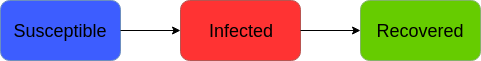
\includegraphics[width=0.7\textwidth]{./fig/SIR_transitions.png}
  
  \begin{itemize}
    \item Population size $N = 1,000$
 	\item Contact rate $\beta = 0.2$
 	\item Infection probability $\gamma = 0.05$
 	\item Illness duration $\delta = 15$
 	\item 1 initially infected agent
  \end{itemize}
    
  \begin{block}{System Dynamics}
    Top-Down, formalised using Differential Equations, give rise to dynamics.
  \end{block}
\end{frame}

\begin{frame}{SIR Model Dynamics}
  \center
  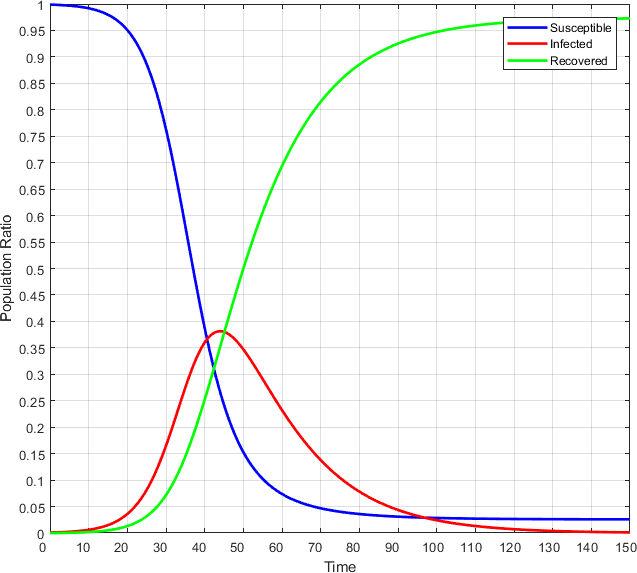
\includegraphics[width=0.7\textwidth]{./fig/SIR_SD_1000agents_150t_001dt.png}
\end{frame}

\begin{frame}{How-To implement ABS?}
  \begin{block}{Established, state-of-the-art approach in ABS}
	Object-Oriented Programming in Python, Java,...
  \end{block}
  
  \begin{block}{We want (pure) functional programming}
	Purity, explicit about side-effects, declarative, reasoning, parallelism, concurrency, property-based testing,...
  \end{block}
  
  \begin{block}{How can we do it?}
  	Functional Reactive Programming
  \end{block}
\end{frame}

\begin{frame}{Functional Reactive Programming (FRP)}
  \begin{itemize}
    \item Continuous- \& discrete-time systems in functional programming
 	\item Signal Function (SF) \\ $\Rightarrow$ process over time, maps signal to signal
 	\item Events (deterministic \& stochastic)
 	\item Random-number streams
 	%\item Running signal-functions in pure way
 	\item \textit{Arrowized} FRP using the \textit{Yampa} library
  \end{itemize}
\end{frame}

\section{Agent-Based SIR in Haskell}
\begin{frame}[fragile]{First Steps}
\begin{minted}[fontsize=\footnotesize, linenos]{haskell}
data SIRState = Susceptible | Infected | Recovered

type SIRAgent = SF [SIRState] SIRState 
  
sirAgent :: RandomGen g => g -> SIRState -> SIRAgent
sirAgent g Susceptible = susceptibleAgent g
sirAgent g Infected    = infectedAgent g
sirAgent _ Recovered   = recoveredAgent
  
recoveredAgent :: SIRAgent
recoveredAgent = arr (const Recovered)
\end{minted}
\end{frame}

\begin{frame}[fragile]{Susceptible Agent}
\begin{minted}[fontsize=\tiny, linenos]{haskell}
susceptibleAgent :: RandomGen g => g -> SIRAgent
susceptibleAgent g = switch (susceptible g) (const (infectedAgent g))
  where
    susceptible :: RandomGen g => g -> SF [SIRState] (SIRState, Event ())
    susceptible g = proc as -> do
      makeContact <- occasionally g (1 / contactRate) () -< ()
      if isEvent makeContact
        then (do
          -- draw random element from the list
          a <- drawRandomElemSF g -< as
          case a of
            Infected -> do
              -- returns True with given probability
              i <- randomBoolSF g infectivity -< ()
              if i
                then returnA -< (Infected, Event ())
                else returnA -< (Susceptible, NoEvent)
             _       -> returnA -< (Susceptible, NoEvent))
        else returnA -< (Susceptible, NoEvent)
\end{minted}
\end{frame}

\begin{frame}[fragile]{Infected Agent}
\begin{minted}[fontsize=\tiny, linenos]{haskell}
infectedAgent :: RandomGen g => g -> SIRAgent
infectedAgent g = switch infected (const recoveredAgent)
  where
    infected :: SF [SIRState] (SIRState, Event ())
    infected = proc _ -> do
      recEvt <- occasionally g illnessDuration () -< ()
      let a = event Infected (const Recovered) recEvt
      returnA -< (a, recEvt)
\end{minted}
\end{frame}

\begin{frame}[fragile]{Running the Simulation}
\begin{minted}[fontsize=\tiny, linenos]{haskell}
runSimulation :: RandomGen g => g -> Time -> DTime -> [SIRState] -> [[SIRState]]
runSimulation g t dt as = embed (stepSimulation sfs as) ((), dts)
  where
    steps     = floor (t / dt)
    dts       = replicate steps (dt, Nothing)
    n         = length as
    (rngs, _) = rngSplits g n [] -- unique rngs for each agent
    sfs       = zipWith sirAgent rngs as
    
stepSimulation :: [SIRAgent] -> [SIRState] -> SF () [SIRState]
stepSimulation sfs as =
    dpSwitch
      -- feeding the agent states to each SF
      (\_ sfs' -> (map (\sf -> (as, sf)) sfs'))
      -- the signal functions
      sfs
      -- switching event, ignored at t = 0         
      (switchingEvt >>> notYet)
      -- recursively switch back into stepSimulation         
      stepSimulation                            
  where
    switchingEvt :: SF ((), [SIRState]) (Event [SIRState])
    switchingEvt = arr (\ (_, newAs) -> Event newAs)
\end{minted}
\end{frame}

%\begin{frame}{Dynamics $\Delta t = 0.1$}
%\begin{figure}
%\begin{center}
%	\begin{tabular}{c c}
%		\begin{subfigure}[b]{0.42\textwidth}
%			\centering
%			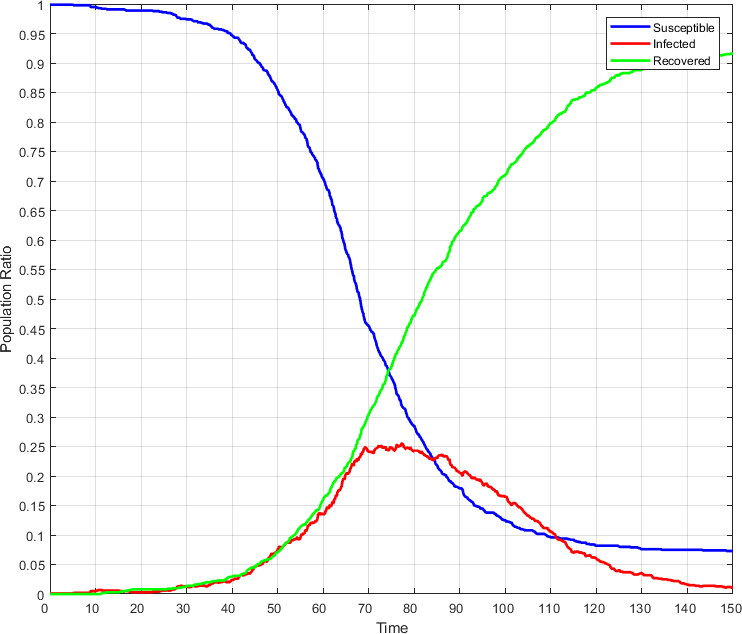
\includegraphics[width=1\textwidth, angle=0]{./fig/SIR_1000agents_150t_01dt.png}
%			\caption{Agent-Based approach}
%		\end{subfigure}
%    	
%    	&
%  
%		\begin{subfigure}[b]{0.4\textwidth}
%			\centering
%			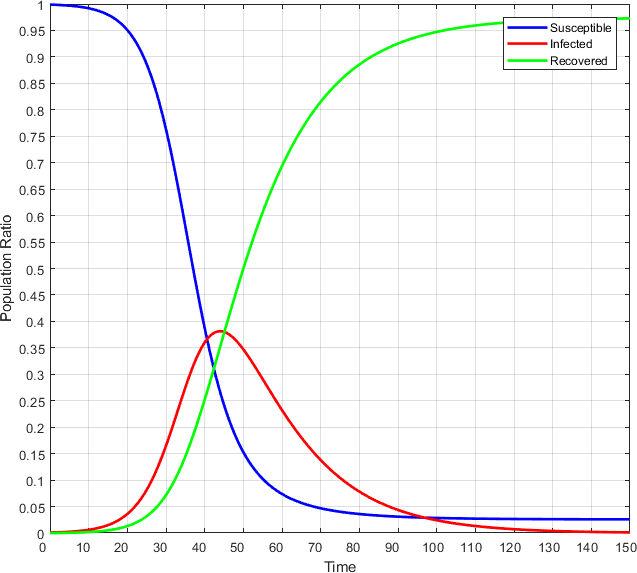
\includegraphics[width=1\textwidth, angle=0]{./fig/SIR_SD_1000agents_150t_001dt.png}
%			\caption{System Dynamics}
%		\end{subfigure}
%	\end{tabular}
%\end{center}
%\end{figure}
%\end{frame}
%
%\begin{frame}{Sampling Issues}
%\begin{figure}
%\begin{center}
%	
\includegraphics[width=0.6\textwidth, angle=0]{./fig/Undersampling.png}
%	\caption*{Undersampling}
%\end{center}
%\end{figure}
%
%\begin{figure}
%\begin{center}
%	
\includegraphics[width=0.6\textwidth, angle=0]{./fig/Supersampling.png}
%	\caption*{Supersampling}
%\end{center}
%\end{figure}
%\end{frame}

\begin{frame}{Dynamics $\Delta t = 0.1$}
\begin{figure}
\begin{center}
	\begin{tabular}{c c}
		\begin{subfigure}[b]{0.42\textwidth}
			\centering
			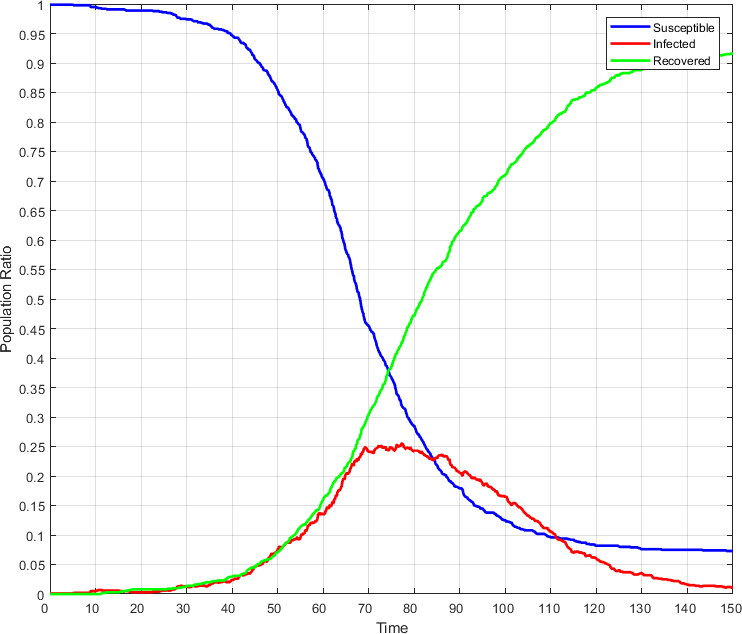
\includegraphics[width=1\textwidth, angle=0]{./fig/SIR_1000agents_150t_01dt.png}
			\caption{Agent-Based approach}
		\end{subfigure}
    	
    	&
  
		\begin{subfigure}[b]{0.4\textwidth}
			\centering
			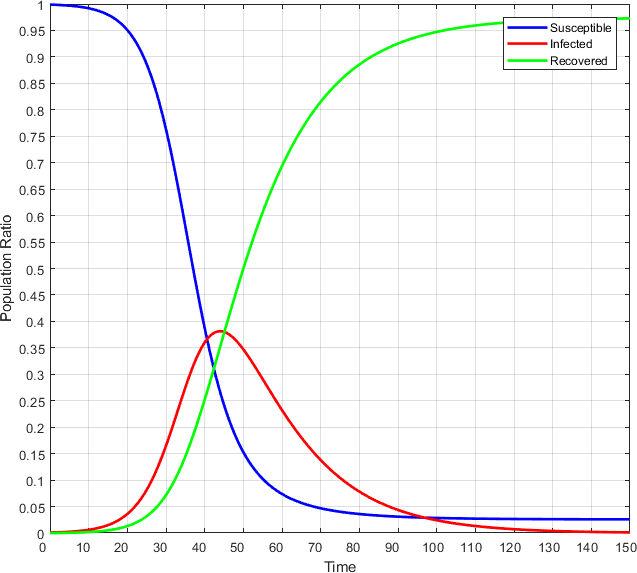
\includegraphics[width=1\textwidth, angle=0]{./fig/SIR_SD_1000agents_150t_001dt.png}
			\caption{System Dynamics}
		\end{subfigure}
	\end{tabular}
\end{center}
\end{figure}
\end{frame}

\begin{frame}{Dynamics $\Delta t = 0.01$}
\begin{figure}
\begin{center}
	\begin{tabular}{c c}
		\begin{subfigure}[b]{0.42\textwidth}
			\centering
			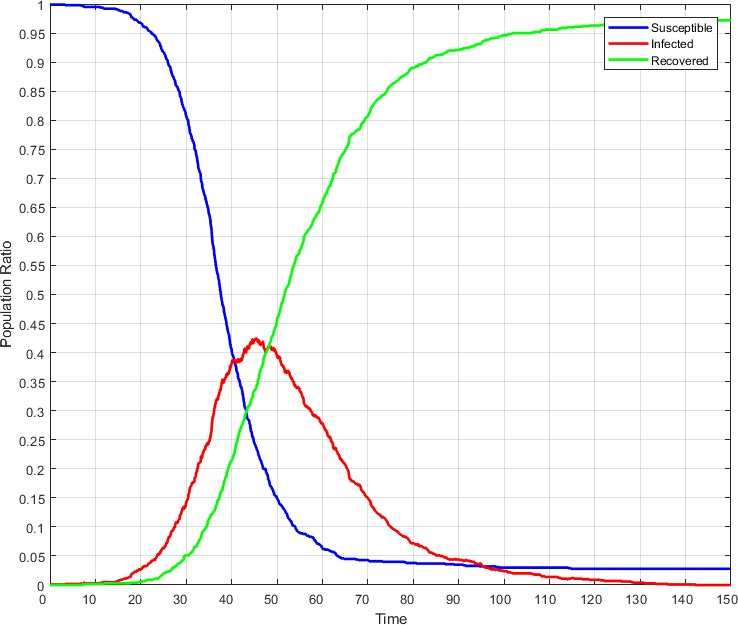
\includegraphics[width=1\textwidth, angle=0]{./fig/SIR_1000agents_150t_001dt.png}
			\caption{Agent-Based approach}
		\end{subfigure}
    	
    	&
  
		\begin{subfigure}[b]{0.4\textwidth}
			\centering
			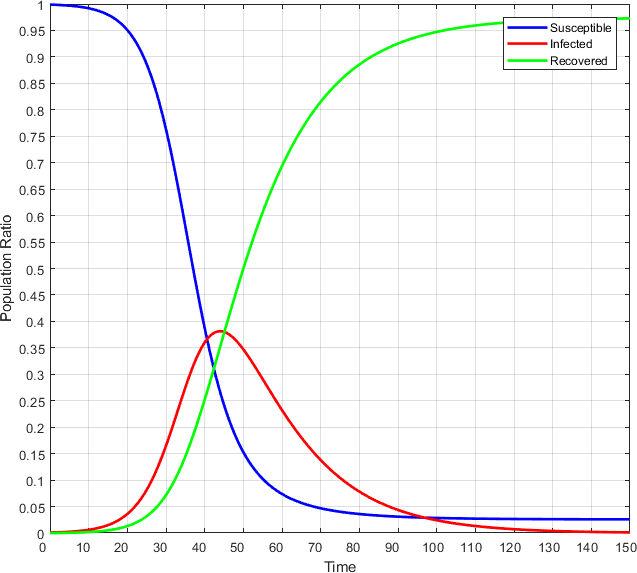
\includegraphics[width=1\textwidth, angle=0]{./fig/SIR_SD_1000agents_150t_001dt.png}
			\caption{System Dynamics}
		\end{subfigure}
	\end{tabular}
\end{center}
\end{figure}
\end{frame}

\begin{frame}{Reflection}
  \begin{itemize}
	\item \textbf{Time} % - simulation over virtual time, modelled explicitly, divided into \textit{fixed} $\Delta t$, at each step all agents executed.
	\item \textbf{Agents} %- implemented as an individual, behaviour depending on internal state.
	\item \textbf{Feedback} %- output state of agent in time-step $t$ is input for next time-step $t + \Delta t$.
	%\item \textbf{Environment} - fully-connected network (complete graph).
	\item \textbf{Stochasticity}
	\item \textbf{Deterministic} %- repeated runs with same initial random-number generator result in same dynamics.
  \end{itemize}
\end{frame}

\section{Adding Spatiality}
\begin{frame}{Where is the Environment?}
  \begin{block}{Adding an Environment}
    \begin{itemize}
      \item Running SFs \textit{'parallel'} \\ $\Rightarrow$ multiple copies of environment
      \item State Monad elegant solution
    \end{itemize}
  \end{block} 
  
  \begin{block}{Problem}
  	\textit{Yampa} not monadic
  \end{block}
  
  \begin{block}{Solution}
    Monadic Stream Functions (MSFs) \\
  	$\Rightarrow$ Signal Functions with monadic context
  \end{block}
\end{frame}

\begin{frame}{The environment: Moore neighbourhood}
  \begin{center}
    
\includegraphics[width=0.5\textwidth]{./fig/moore.png}
  \end{center}
\end{frame}

\begin{frame}[fragile]{Re-defining Types}
\begin{minted}[fontsize=\tiny, linenos]{haskell}
type Disc2dCoord = (Int, Int)
type SIREnv      = Array Disc2dCoord SIRState

type SIRMonad g = StateT SIREnv (Rand g)
type SIRAgent g = SF (SIRMonad g) () ()

neighbours :: SIREnv -> Disc2dCoord -> Disc2dCoord -> [Disc2dCoord] -> [SIRState]

moore :: [Disc2dCoord]
moore = [ topLeftDelta,    topDelta,     topRightDelta,
          leftDelta,                     rightDelta,
          bottomLeftDelta, bottomDelta,  bottomRightDelta ]

topLeftDelta :: Disc2dCoord
topLeftDelta      = (-1, -1)

topDelta :: Disc2dCoord
topDelta          = ( 0, -1)
...
\end{minted}
\end{frame}

\begin{frame}[fragile]{Susceptible Agent revisited}
\begin{minted}[fontsize=\tiny, linenos]{haskell}
susceptibleAgent :: RandomGen g => Disc2dCoord -> SIRAgent g
susceptibleAgent coord = switch susceptible (const (infectedAgent coord))
  where
    susceptible :: RandomGen g => SF (SIRMonad g) () ((), Event ())
    susceptible = proc _ -> do
      makeContact <- occasionallyM (1 / contactRate) () -< ()
      if not (isEvent makeContact)
        then returnA -< ((), NoEvent)
        else (do
          env <- arrM_ (lift get) -< ()
          let ns = neighbours env coord agentGridSize moore
          s <- drawRandomElemS -< ns
          case s of
            Infected -> do
              infected <- arrM_ 
                (lift $ lift $ randomBoolM infectivity) -< ()
              if infected 
                then (do
                  arrM (put . changeCell coord Infected) -< env
                  returnA -< ((), Event ()))
                else returnA -< ((), NoEvent)
            _        -> returnA -< ((), NoEvent))
\end{minted}
\end{frame}

%\begin{frame}[fragile]{Running the Simulation revisited}
%\begin{minted}[fontsize=\tiny, linenos]{haskell}
%runSimulation :: RandomGen g
%              => g -> Time -> DTime -> SIREnv -> [(Disc2dCoord, SIRState)] -> [SIREnv]
%runSimulation g t dt env as = evalRand esRand g
%  where
%    steps    = floor (t / dt)
%    dts      = replicate steps ()
%    -- initial SFs of all agents
%    sfs      = map (uncurry sirAgent) as   
%    -- running the simulation   
%    esReader = embed (stepSimulation sfs) dts 
%    esState  = runReaderT esReader dt 
%    esRand   = evalStateT esState env   
%    
%stepSimulation :: RandomGen g => [SIRAgent g] -> SF (SIRMonad g) () SIREnv
%stepSimulation sfs = MSF (\_ -> do
%  -- running all SFs with unit input
%  res <- mapM (`unMSF` ()) sfs
%  -- extracting continuations, ignore output
%  let sfs' = fmap snd res
%  -- getting environment of current step   
%  env <- get
%  -- recursive continuation    
%  let ct = stepSimulation sfs'  
%  return (env, ct))
%\end{minted}
%\end{frame}

\begin{frame}{Dynamics with environment}
\begin{figure}
\begin{center}
	\begin{tabular}{c c}
		\begin{subfigure}[b]{0.47\textwidth}
			\centering
			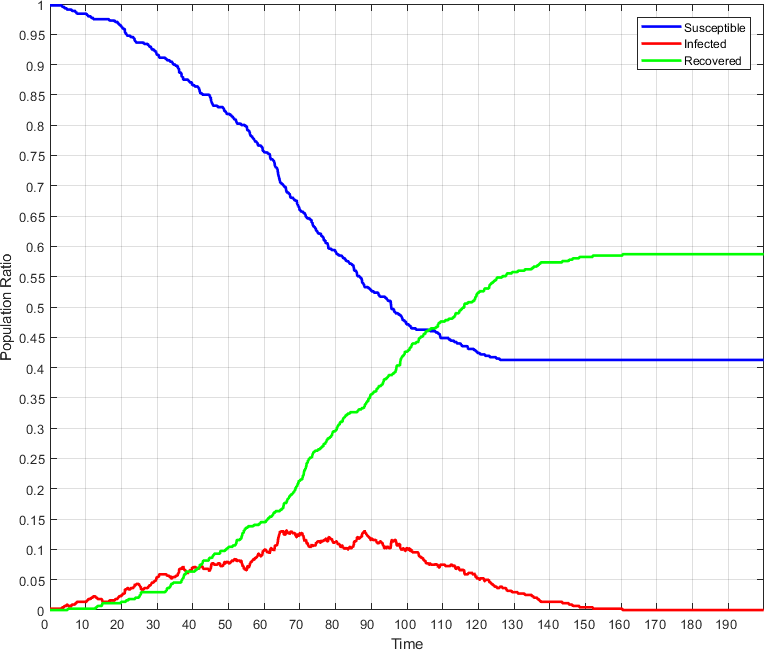
\includegraphics[width=1\textwidth, angle=0]{./fig/SIR_dynamics_30x30agents_300t_01dt.png}
			\caption{Dynamics over $t = 200$}
		\end{subfigure}
    	
    	&
  
		\begin{subfigure}[b]{0.4\textwidth}
			\centering
			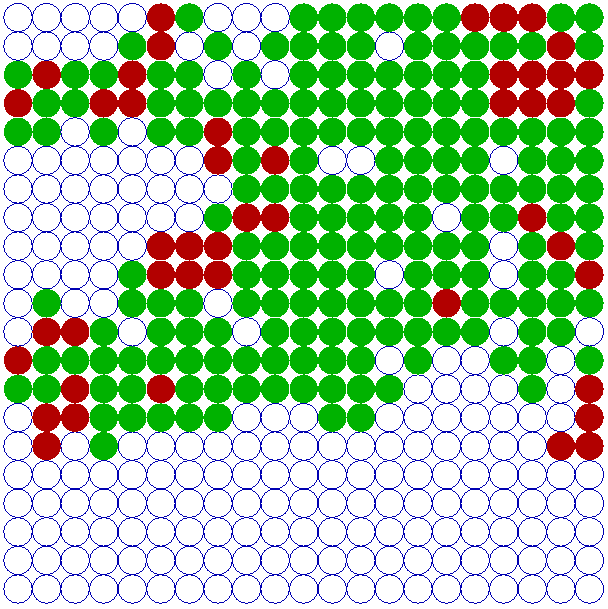
\includegraphics[width=1\textwidth, angle=0]{./fig/SIR_environment_30x30agents_t100_01dt.png}
			\caption{Visualisation at $t = 100$}
		\end{subfigure}
	\end{tabular}
\end{center}
\end{figure}
\end{frame}

\section{Discussion}
%\begin{frame}{Performance}
%  \begin{block}{Experiment}
%    Spatial Agent-Based SIR, 51x51 Grid (2,601 agents), $t = 100$, $\Delta t = 0.1$, avg. 8 runs
%  \end{block}
%  
%  \begin{block}{Haskell}
%  	100.3 sec
%  \end{block}
%  
%  \begin{block}{RePast ($\Delta t = ?$)}
%  	10.8 sec
%  \end{block}
%  
%  \begin{block}{STM Haskell}
%  	8.6 sec on Amazon S2, 16 cores (other paper)
%  \end{block}
%\end{frame}

\begin{frame}{Conclusion}
  \begin{itemize}
    \item Purity guarantees reproducibility at compile time
    \item Performance
    \item Agent-Identity a bit lost
    \item Agent-Interaction is main difficulty
  \end{itemize}
\end{frame}

\begin{frame}{Future Work}
  \begin{block}{Property-based testing for verification in ABS}
    Might offer huge benefits e.g. formalising hypotheses
  \end{block}
  
  \begin{block}{Dependent Types in ABS (using Idris)}
  	\begin{itemize}
  	  \item Safe environment access, state-transitions, agent-interactions
      \item Equilibrium of Model \& Totality of Implementation
  	\end{itemize}
  \end{block}
\end{frame}

\begin{frame}{}
  \begin{center}
  Thank You!
  \end{center}
\end{frame}
\end{document}